\documentclass[11pt]{amsart}
\usepackage[margin=1.05in]{geometry}
\usepackage{amssymb,booktabs,xcolor,tikz}
\usetikzlibrary{arrows.meta,positioning,calc}
\usepackage[colorlinks,urlcolor=blue,citecolor=blue,linkcolor=blue]{hyperref}
\newtheorem{theorem}{Theorem}[section]
\newtheorem{lemma}[theorem]{Lemma}
\newtheorem{proposition}[theorem]{Proposition}
\newtheorem{corollary}[theorem]{Corollary}
\theoremstyle{definition}
\newtheorem{definition}[theorem]{Definition}
\theoremstyle{remark}
\newtheorem{remark}[theorem]{Remark}
\newcommand{\R}{\mathbb R}
\newcommand{\Z}{\mathbb Z}
\newcommand{\Q}{\mathbb Q}
\newcommand{\low}{\mathrm{low}}
\newcommand{\high}{\mathrm{high}}
\newcommand{\gap}{\mathrm{gap}}
\newcommand{\opt}{\mathrm{opt}}
\newcommand{\Bx}{\mathrm{Bx}}

\title{The Tight-Tile Lemma for the $k^2-5$ family: statement and proof}
\author{Mohsen Khalili}
\address{Independent researcher}
\email{mkhalili63@yahoo.com}
\author{Sara Gharabaghi}
\address{Independent researcher}
\date{Technical report accompanying ``$k^2-5$ unit squares need a square of side $k$ for every $k\ge7$'';
November 12, 2026}

\begin{document}
\begin{abstract}
We give the full statement and proof of the Tight-Tile Lemma used in the companion paper to show that the measure
$\mu_{11}$ of the $k^2-5$ family is valid on $[0,11]^2$. The lemma concerns unit squares near \emph{tight tiles}:
axis-parallel unit squares next to a wall whose mass, as a limit at zero tilt, is exactly $1$. The proof blows up
the neighborhood of each tile with the tilt as scale variable, bounds the mass on each cell of the blown-up space
from below by a concave function built from exact limit values and interval-certified derivative bounds, and checks
this bound at the cell's vertices in exact rational arithmetic. We state every lemma used, describe the program
\texttt{ttbox} that carries out the case analysis, list its soundness rules, and report the computation, the
coverage check, controls and an independent review.
\end{abstract}
\maketitle
\tableofcontents

\section{Setting}\label{sec:setting}

\subsection{The measure}
$\mu=\mu_{11}$ is the measure on $[0,11]^2$ given by the file \texttt{sol\_exact\_box11.txt} (SHA-256
\texttt{d259fed5\ldots adbd12099}, full hash in the release). It is the sum of
\begin{itemize}
\item $13{,}244$ axis-parallel segments $\gamma_i=\{g_i+\tau(g_i'-g_i):\tau\in[0,1]\}$, $g_i,g_i'\in\frac1{10}\Z^2$,
each with weight $w_i>0$ (the mass of the whole segment, spread uniformly by length; the smallest weight is
$1.01\cdot10^{-10}$), and
\item Lebesgue measure on $U=[\frac{19}5,\frac{36}5]^2$.
\end{itemize}
$\mu$ is invariant under the eight symmetries of $[0,11]^2$ (checked in exact arithmetic).

\subsection{Poses}
For a center $c\in\R^2$ and an angle $\theta$, let $u=\tan(\theta/2)$, $N=1+u^2$ and
\[
e_1=\Bigl(\frac{1-u^2}N,\ \frac{2u}N\Bigr),\qquad e_2=\Bigl(-\frac{2u}N,\ \frac{1-u^2}N\Bigr).
\]
The pose is the closed unit square $P(c,u)=\{z\in\R^2:|(z-c)\cdot e_1|\le\frac12,\ |(z-c)\cdot e_2|\le\frac12\}$, and
\[
\mu(P)=\sum_i w_i\,\ell_i(P)+|P\cap U|,\qquad \ell_i(P)=\bigl|\{\tau\in[0,1]:g_i+\tau(g_i'-g_i)\in P\}\bigr|.
\]

\subsection{Tight tiles}
By symmetry we treat the left wall $x=0$. The tile at depth $j\in\{1,2,3\}$ and height $y$ is the axis-parallel unit
square with center $(d_0,y)$, $d_0=j+\frac12$. A pose near it is written with center $(d_0+\delta,\,y)$ and
$\tan(\theta/2)=\sigma u$, where $\sigma\in\{+1,-1\}$ is the \emph{tilt sign} and $u>0$.

\begin{figure}[ht]
\centering% Figure: a tight tile next to the left wall and a slightly tilted pose near it (tilt exaggerated)
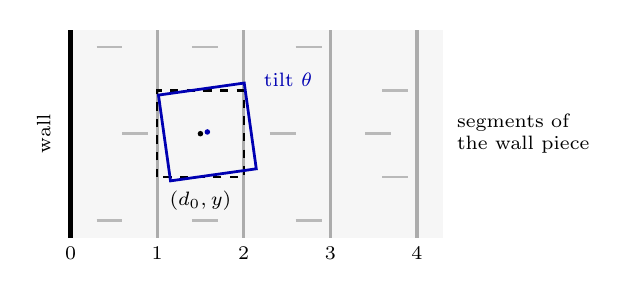
\begin{tikzpicture}[x=1.1cm,y=1.1cm,font=\scriptsize]
  \fill[gray!7] (0,-1.2) rectangle (4.3,1.2);
  \draw[line width=1.5pt] (0,-1.2) -- (0,1.2);
  \node[below] at (0,-1.2) {$0$};
  \foreach \x in {1,2,3,4} {\draw[gray!65,line width=1.1pt] (\x,-1.2) -- (\x,1.2); \node[below] at (\x,-1.2) {$\x$};}
  \foreach \y/\x in {-1/0.3,-1/1.4,-1/2.6,0/0.6,0/2.3,0/3.4,1/0.3,1/1.4,1/2.6,-0.5/3.6,0.5/3.6} \draw[gray!55,line width=0.9pt] (\x,\y) -- ++(0.3,0);
  \draw[dashed,line width=0.9pt] (1,-0.5) rectangle (2,0.5);
  \begin{scope}[shift={(1.58,0.02)},rotate=8]
    \draw[blue!70!black,line width=1pt] (-0.5,-0.5) rectangle (0.5,0.5);
  \end{scope}
  \fill (1.5,0) circle (1pt); \fill[blue!70!black] (1.58,0.02) circle (1pt);
  \node[below] at (1.5,-0.55) {$(d_0,y)$};
  \node[blue!70!black,right] at (2.12,0.62) {tilt $\theta$};
  \node[left,rotate=90,anchor=south] at (-0.12,0) {wall};
  \node[right,align=left] at (4.35,0) {segments of\\the wall piece};
\end{tikzpicture}

\caption{A tight tile at depth $1$ (dashed) and a nearby pose with center $(d_0+\delta,y)$ and tilt $\theta$ (blue,
tilt exaggerated). In the limit $\theta\to0$ the tile's mass is exactly $1$.}
\label{fig:tile}
\end{figure}

\subsection{Parameters}
$K=4$, $M=4$, $u_0=1/4000$, $\delta_{\max}=Ku_0=1/1000$, and the height ranges
\begin{align*}
I(3/2)&=[1.4,1.7]\cup[2.4,2.7]\cup[3.3,5.5],\\
I(5/2)&=[1.4,1.7]\cup[2.3,2.7]\cup[3.3,3.7]\cup[3.8,5.5],\\
I(7/2)&=[1.4,1.7]\cup[2.3,2.7]\cup[3.3,3.7]\cup[4.1,4.5].
\end{align*}
On five further ranges (Table~\ref{tab:u2000}) we use $u_0=1/2000$ and $\delta_{\max}=1/500$.

\begin{table}[h]
\begin{tabular}{lll}
\toprule
$d_0$ & $\sigma$ & ranges of $y$ with $u_0=1/2000$\\
\midrule
$3/2$ & $+1$ & $[4.2,4.3]$, $[4.5,4.6]$\\
$3/2$ & $-1$ & $[3.8,3.9]$, $[5.4,5.5]$\\
$5/2$ & $-1$ & $[4.4,4.5]$\\
\bottomrule
\end{tabular}
\caption{Ranges certified with the larger tilt bound.}\label{tab:u2000}
\end{table}

\section{Statement}\label{sec:statement}

\begin{theorem}[Tight-Tile Lemma]\label{thm:tt}
Let $d_0\in\{3/2,5/2,7/2\}$, $\sigma\in\{+1,-1\}$ and $y\in I(d_0)$. Every pose with center $(d_0+\delta,y)$ and
$\tan(\theta/2)=\sigma u$, where $0<u\le u_0$ and $|\delta|\le\delta_{\max}$, has $\mu(P)\ge1$. The same holds with
$u_0=1/2000$ and $\delta_{\max}=1/500$ for the ranges of Table~\ref{tab:u2000}, each extended by $1/500$ at both
ends.
\end{theorem}

\begin{remark}[how the lemma is used]
The interval checker \texttt{zmx2} certifies all poses of $[0,11]^2$ except the sub-boxes it leaves in $76$ root
boxes. One of them (root $9632$) is closed by the exact checker \texttt{qx2\_zm.py}. The other $75$ are neighborhoods of
tight tiles, and Section~\ref{sec:coverage} shows that every sub-box left there consists of poses covered by
Theorem~\ref{thm:tt} or of untilted poses ($u=0$), which are certified separately.
\end{remark}

\section{Exact chords}\label{sec:chords}

\begin{lemma}[clip formula]\label{lem:clip}
For a segment $\gamma=\{g+\tau(g'-g)\}$, each of the four half-planes of $P(c,u)$ reads $\tau A\le B$ with
\[
A=s\,(g'-g)\cdot Ne_i,\qquad B=\tfrac N2-s\,(g-c)\cdot Ne_i,\qquad i\in\{1,2\},\ s\in\{+1,-1\}.
\]
Let $\mathcal B^+$ consist of $1$ and the ratios $B/A$ with $A>0$, and $\mathcal B^-$ of $0$ and the ratios with
$A<0$. If some constraint has $A=0$ and $B<0$, then $\ell=0$; constraints with $A=0\le B$ hold for all $\tau$. Otherwise
\[
\ell(P)=\max\bigl(0,\ \min\mathcal B^+-\max\mathcal B^-\bigr).
\]
\end{lemma}

\begin{proof}
$|(z-c)\cdot e_i|\le\frac12$ is the pair of inequalities $s(z-c)\cdot e_i\le\frac12$. Substituting
$z=g+\tau(g'-g)$ and multiplying by $N>0$ gives $\tau A\le B$. The set of $\tau\in[0,1]$ satisfying all four is the
interval $[\max\mathcal B^-,\min\mathcal B^+]$ (empty if the bounds cross).
\end{proof}

With the factor $N$, the quantities $A$ and $B$ are polynomials in $u$ and $c$ with rational coefficients.

\section{Charts}\label{sec:charts}

Throughout, the scale variable is the tilt: $h=u$. In each chart the pose has
\[
c=c_0(p,q)+h\,c_1(p,q,h),\qquad \tan(\theta/2)=\sigma h,
\]
with $c_0$ affine and $c_1$ polynomial in the \emph{face coordinates} $(p,q)$, so $A$ and $B$ are polynomials in
$(p,q,h)$ with rational coefficients.

\begin{lemma}[division]\label{lem:division}
Let $h^m$ be the largest power of $h$ dividing both $A$ and $B$. On the region $h>0$, the constraint $\tau A\le B$ is
equivalent to $\tau(A/h^m)\le B/h^m$.
\end{lemma}

\begin{proof}
$h^m>0$.
\end{proof}

\subsection{Charts near a base line}
Let $y_b\in\frac1{10}\Z$ and $t=y-y_b$. The neighborhood of the line is
$\mathcal V(y_b)=\{0<u\le u_0,\ |t|\le Ku_0,\ |\delta|\le\delta_{\max}\}$.

\begin{table}[h]
\begin{tabular}{llll}
\toprule
chart & poses & face coordinates $(p,q)$ & slab \\
\midrule
$C_u$ & $|\delta|,|t|\le Ku$ & $(\delta/u,\ t/u)\in[-K,K]^2$ & $0\le h\le u_0$\\
$W_t^\pm$ & $|\delta|\le Ku<|t|$, $\pm t>0$ & $(\delta/u,\ |t|)\in[-K,K]\times[0,Ku_0]$ & $h\le|t|/K$\\
$W_d^\pm$ & $|t|\le Ku<|\delta|$, $\pm\delta>0$ & $(t/u,\ |\delta|)\in[-K,K]\times[0,\delta_{\max}]$ & $h\le|\delta|/K$\\
$W_{td}^{\pm\pm}$ & $Ku<|\delta|$, $Ku<|t|$ & $(|t|,|\delta|)$, triangles $|t|\le|\delta|$ or $|\delta|\le|t|$ &
$h\le\min(|t|,|\delta|)/K$\\
\bottomrule
\end{tabular}
\caption{Charts near the base line $y_b$.}\label{tab:charts}
\end{table}

\subsection{Strip charts}
For $y\in[y_b+Ku_0,\,y_b+\frac1{10}-Ku_0]$: $\Sigma_u$ with face $(\delta/u,\,y)$ for $|\delta|\le Ku$ and slab $h\le u_0$;
and $\Sigma_d^\pm$ with face $(y,\,|\delta|)$ for $\pm\delta>Ku$ and slab $h\le|\delta|/K$.

\begin{lemma}[the charts cover]\label{lem:charts}
Every pose of Theorem~\ref{thm:tt} lies in one of these charts, with face coordinates in the stated ranges and $h=u$
in the stated slab.
\end{lemma}

\begin{proof}
Each $I(d_0)$, and each range of Table~\ref{tab:u2000}, is a finite union of intervals $[y_1,y_2]$ with
$y_1,y_2\in\frac1{10}\Z$. Each $y$ in such an interval satisfies $|y-y_b|\le Ku_0$ for a line
$y_b\in\frac1{10}\Z\cap[y_1,y_2]$, or lies in a strip between consecutive lines of the interval. Near a line,
$|t|\le Ku_0$ and $|\delta|\le\delta_{\max}=Ku_0$, and exactly one of the four cases of Table~\ref{tab:charts} holds.
In $C_u$, $(p,q)=(\delta/u,t/u)\in[-K,K]^2$ and $h=u\le u_0$. In $W_t^\pm$, $p=\delta/u\in[-K,K]$,
$q=|t|\le Ku_0$ and $h=u<|t|/K$; $W_d^\pm$ is symmetric. In $W_{td}$, $h<\min(|t|,|\delta|)/K$. In a strip the same
split by $|\delta|\le Ku$ or $>Ku$ gives $\Sigma_u$ or $\Sigma_d^\pm$. For the ranges of Table~\ref{tab:u2000}, the
charts of the two end lines also cover heights within $Ku_0=1/500$ beyond the range, which gives the extension.
\end{proof}

\begin{figure}[ht]
\centering% Figure: the four-way splits. (a) charts near a base line in the (delta, t) plane at a fixed tilt u;
% (b) the zones around a corner point of a face; (c) wedge-corner zones and the ray zones.
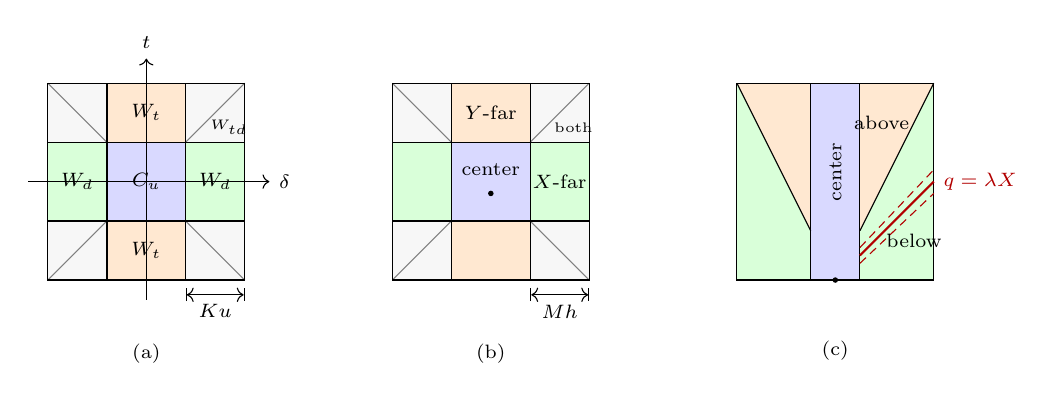
\begin{tikzpicture}[font=\scriptsize,x=1.25cm,y=1.25cm]
 \def\ttfourway{%
  \fill[gray!6] (-1,-1) rectangle (1,1);
  \fill[blue!15] (-0.4,-0.4) rectangle (0.4,0.4);
  \fill[orange!18] (-0.4,0.4) rectangle (0.4,1); \fill[orange!18] (-0.4,-1) rectangle (0.4,-0.4);
  \fill[green!15] (0.4,-0.4) rectangle (1,0.4); \fill[green!15] (-1,-0.4) rectangle (-0.4,0.4);
  \foreach \sx in {1,-1} \foreach \sy in {1,-1} \draw[gray] (0.4*\sx,0.4*\sy) -- (\sx,\sy);
  \draw (-1,-1) rectangle (1,1); \draw (-0.4,-1) -- (-0.4,1) (0.4,-1) -- (0.4,1) (-1,-0.4) -- (1,-0.4) (-1,0.4) -- (1,0.4);}
 \begin{scope}
  \ttfourway
  \node at (0,0) {$C_u$}; \node at (0,0.7) {$W_t$}; \node at (0,-0.7) {$W_t$}; \node at (0.7,0) {$W_d$}; \node at (-0.7,0) {$W_d$};
  \node[font=\tiny] at (0.84,0.55) {$W_{td}$};
  \draw[->] (-1.2,0) -- (1.25,0) node[right] {$\delta$}; \draw[->] (0,-1.2) -- (0,1.25) node[above] {$t$};
  \draw[|<->|] (0.4,-1.15) -- node[below] {$Ku$} (1,-1.15);
  \node at (0,-1.75) {(a)};
 \end{scope}
 \begin{scope}[shift={(3.5,0)}]
  \ttfourway
  \node at (0,0.12) {center}; \node at (0,0.7) {$Y$-far}; \node at (0.7,0) {$X$-far}; \node[font=\tiny] at (0.84,0.55) {both};
  \fill (0,-0.12) circle (1pt);
  \draw[|<->|] (0.4,-1.15) -- node[below] {$Mh$} (1,-1.15);
  \node at (0,-1.75) {(b)};
 \end{scope}
 \begin{scope}[shift={(7.0,-1)},y=2.5cm]
  \fill[gray!6] (-1,0) rectangle (1,1);
  \fill[blue!15] (-0.25,0) rectangle (0.25,1);
  \fill[green!15] (0.25,0) -- (1,0) -- (1,1) -- (0.25,0.25) -- cycle; \fill[green!15] (-0.25,0) -- (-1,0) -- (-1,1) -- (-0.25,0.25) -- cycle;
  \fill[orange!18] (0.25,0.25) -- (1,1) -- (0.25,1) -- cycle; \fill[orange!18] (-0.25,0.25) -- (-1,1) -- (-0.25,1) -- cycle;
  \draw (-1,0) rectangle (1,1); \draw (-0.25,0) -- (-0.25,1) (0.25,0) -- (0.25,1);
  \draw (0.25,0.25) -- (1,1) (-0.25,0.25) -- (-1,1);
  \draw[red!70!black,thick] (0.25,0.125) -- (1,0.5);
  \draw[red!70!black,densely dashed] (0.25,0.085) -- (1,0.44) (0.25,0.165) -- (1,0.56);
  \node[rotate=90] at (0,0.55) {center};
  \node at (0.47,0.8) {above}; \node at (0.8,0.2) {below};
  \node[red!70!black,right] at (1,0.5) {$q=\lambda X$};
  \fill (0,0) circle (1pt);
  \node at (0,-0.36) {(c)};
 \end{scope}
\end{tikzpicture}

\caption{(a) The charts of Table~\ref{tab:charts} in the $(\delta,t)$ plane at a fixed tilt $u$. (b) The zones around a
corner point of $C_u$ (Section~\ref{sec:corners}), at a fixed $h$. (c) The zones around a corner point of a wedge chart,
and the near zone (dashed) around a ray $q=\lambda X$.}
\label{fig:zones}
\end{figure}

A chart whose slab is $h\le\chi\,\xi$ for a face coordinate $\xi\ge0$ and a constant $\chi>0$ is a \emph{wedge chart}
with wedge variable $\xi$.

\section{The bound on a cell}\label{sec:cell}

\begin{definition}
A \emph{cell} is $Z=\{(p,q,h):(p,q)\in\Pi,\ \low(p,q)\le h\le\high(p,q)\}$, where $\Pi$ is a convex polygon with
rational vertices and $0\le\low\le\high$ are affine. Its \emph{box} is $\Bx(Z)=\mathrm{bbox}(\Pi)\times[0,\max_\Pi\high]$.
\end{definition}

\begin{lemma}[vertices]\label{lem:vertices}
$Z$ is a convex polytope whose vertices are among the points $(v,\low(v))$ and $(v,\high(v))$, $v$ a vertex of
$\Pi$.
\end{lemma}

\begin{proof}
$Z$ is an intersection of half-spaces. A point $(z,h)$ of $Z$ with $\low(z)<h<\high(z)$ is interior to a vertical
segment in $Z$, and a point with $z$ not a vertex of $\Pi$ is interior to a segment in $\Pi$ along which $\low$ (or
$\high$) is affine; neither is a vertex.
\end{proof}

\subsection{Classifying constraints}
All enclosures below are computed in binary64 interval arithmetic with outward rounding (Section~\ref{sec:impl}),
on $\Bx(Z)$. For each constraint $\tau A\le B$ (after Lemma~\ref{lem:division}) one of the following is established;
otherwise the cell is refused and split.
\begin{itemize}
\item \emph{Regular}: $A$ has constant sign on $\Bx(Z)$, so $B/A$ is $C^1$ there. In addition $A(p,q,0)$ is a nonzero
constant and $B(p,q,0)$ is affine in $(p,q)$.
\item \emph{Inactive}: $B\ge\max(0,A)$ on $\Bx(Z)$; then $\tau A\le B$ for all $\tau\in[0,1]$.
\item \emph{Empty}: $B<\min(0,A)$ on $\Bx(Z)$; then $\tau A>B$ for all $\tau\in[0,1]$, so the chord is $0$.
\item \emph{Wedge test} (wedge charts, when the two previous tests are inconclusive). Substitute $h=\eta\,\xi$ with
$\eta\in[0,\chi]$, which is exact on the cell, divide $B$ and $B-A$ by the largest power of $\xi$ (positive), and
decide inactive or empty from the signs of both. Near the apex of a wedge, one of two further exact substitutions is
made: $\xi=\zeta\,\xi'$ with $\zeta\in[0,\zeta_{\max}]$ on a region where $\xi\le\zeta_{\max}\xi'$ (the chart provides
$\zeta_{\max}$, by default $1$), or $\xi'=\zeta\,\xi$ with $\zeta\in[-1,1]$ on a region where $|\xi'|\le\xi$.
\end{itemize}

\begin{lemma}[bisection of auxiliary variables]\label{lem:bisect}
If an interval test on the box of $(p,q,\eta,\zeta)$ is inconclusive, the checker bisects the widest of the ranges of
$\eta,\zeta$ (up to $8$ levels) and accepts a verdict only if it is the same, inactive or empty, on every piece. This
verdict holds on the whole box.
\end{lemma}

\begin{proof}
The pieces are closed intervals covering the range, so every point lies in a piece where the verdict holds.
\end{proof}

\subsection{Limit values and mean-value bounds}
For a regular constraint the \emph{limit value} $b(0)=B(p,q,0)/A(p,q,0)$ is affine on $\Pi$. For each segment, write
$b_r^+$ for the ratios $B/A$ of its regular constraints with $A>0$ together with the constant bound $1$, and $b_r^-$
for those with $A<0$ together with the constant bound $0$; a constant bound has derivative $0$, inactive constraints
are dropped, and a segment with an empty constraint contributes $0$ on the whole cell. The checker splits $\Pi$ exactly along affine lines
until, on all of $\Pi$ (checked at the vertices of $\Pi$, which suffices for affine functions), the minimizing upper
bound $b^+_{r_*}(0)$, the maximizing lower bound $b^-_{r_*}(0)$ and the sign of $f(0)=b^+_{r_*}(0)-b^-_{r_*}(0)$ are fixed.

Let $\alpha_r$ and $\beta_r$ be outward-rounded enclosures with
\[
\alpha_r\le\inf_{\Bx(Z)}\partial_h b_r^+,\qquad \beta_r\ge\sup_{\Bx(Z)}\partial_h b_r^-,\qquad
\partial_h\frac BA=\frac{A\,\partial_hB-B\,\partial_hA}{A^2}.
\]

\begin{lemma}[mean value]\label{lem:mvt}
For every $(p,q,h)\in Z$: $b_r^+(h)\ge b_r^+(0)+h\,\alpha_r$ and $b_r^-(h)\le b_r^-(0)+h\,\beta_r$.
\end{lemma}

\begin{proof}
The vertical segment $\{(p,q)\}\times[0,h]$ lies in $\Bx(Z)$, where $b_r^\pm$ is $C^1$; apply the mean value
theorem.
\end{proof}

\begin{lemma}[concave chord bound]\label{lem:concave}
Let $\gap^+_r=b_r^+(0)-b_{r_*}^+(0)\ge0$, $\gap^-_r=b_{r_*}^-(0)-b_r^-(0)\ge0$ and
\[
\varphi=\min_r(\gap^+_r+h\,\alpha_r)+\min_r(\gap^-_r-h\,\beta_r).
\]
Then $\varphi$ is concave in $(p,q,h)$, and with $f(h)=\min\mathcal B^+-\max\mathcal B^-$ and $\ell=\max(0,f)$,
\[
\ell(h)-\ell(0)\ge\max(\opt_0,\opt_1),\quad
\begin{cases}\opt_0=\varphi,\ \opt_1=-f(0)&\text{if }f(0)\ge0\text{ on }\Pi,\\
\opt_0=f(0)+\varphi,\ \opt_1=0&\text{if }f(0)\le0\text{ on }\Pi.\end{cases}
\]
For $\kappa\in[0,1]$, $\kappa\,\opt_1+(1-\kappa)\opt_0$ is concave and is a lower bound for $\ell(h)-\ell(0)$.
\end{lemma}

\begin{proof}
The gaps are affine, so $\varphi$ is a sum of minima of affine functions. By Lemma~\ref{lem:mvt},
$\min\mathcal B^+(h)\ge b^+_{r_*}(0)+\min_r(\gap_r^++h\alpha_r)$ and $\max\mathcal B^-(h)\le
b^-_{r_*}(0)-\min_r(\gap^-_r-h\beta_r)$, so $f(h)\ge f(0)+\varphi$. If $f(0)\ge0$ then $\ell(0)=f(0)$, so
$\ell(h)-\ell(0)\ge\varphi$ and $\ge-f(0)$. If $f(0)\le0$ then $\ell(0)=0$, $\ell(h)\ge f(0)+\varphi$ and
$\ell(h)\ge0$. A convex combination of two lower bounds is at most their maximum; a convex combination of concave
functions is concave.
\end{proof}

\subsection{The Lebesgue term}
Only the depth-$7/2$ tiles reach $U$. Let $a(h)=|P\cap U|$.
\begin{itemize}
\item \emph{Limit value.} At $h=0$ the pose is axis-parallel and $a(0)=A_x(p,q)A_y(p,q)$, where $A_x,A_y$ are the
lengths of the projections of $P\cap U$, which are clamped affine functions of $(p,q)$. The polygon is split at
their kinks, so both are affine on $\Pi$. If both vary, the McCormick bound
$A_xA_y\ge A_x^{\min}A_y+A_xA_y^{\min}-A_x^{\min}A_y^{\min}$ is used; it is affine and valid since
$(A_x-A_x^{\min})(A_y-A_y^{\min})\ge0$.
\item \emph{Derivative.} $a$ is Lipschitz in $h$, and for almost every $h$, by the transport formula with $U$ fixed,
$a'(h)=\int_{\partial P\cap U}v\cdot n\,ds$, where $v$ is the velocity of the boundary point and $n$ the outer normal.
On an edge of $P$ with parameter $s\in[-\frac12,\frac12]$, $v\cdot n=c'\cdot n+\theta'\,\epsilon\,s$ with $\epsilon=\pm1$ fixed by
the edge. The part of the edge in $U$ is an interval $[s_{lo},s_{hi}]$ obtained by clipping the edge against the four
lines of $U$ exactly as in Lemma~\ref{lem:clip} (including Lemma~\ref{lem:division} and the wedge test). The integral
equals $(s_{hi}-s_{lo})\,c'\cdot n+\theta'\epsilon\,(s_{hi}^2-s_{lo}^2)/2$ and is enclosed by intervals; if the edge may miss
$U$, the enclosure is widened to contain $0$. The sum over the four edges gives a lower bound $\alpha_U$ for $a'$ on
$\Bx(Z)$, and $a(h)\ge a(0)+h\,\alpha_U$.
\end{itemize}

\begin{proposition}[cell certificate]\label{prop:cell}
Let $G(p,q)$ be the exact affine limit value of $\mu(P)-1$ on $\Pi$ (with the McCormick bound for the Lebesgue part),
let $\kappa_i\in[0,1]$ be rational, one per segment, and
\[
T=G+\sum_iw_i\bigl(\kappa_i\opt_{1,i}+(1-\kappa_i)\opt_{0,i}\bigr)+h\,\alpha_U .
\]
Then $\mu(P)-1\ge T$ on $Z$ and $T$ is concave. Hence if $T\ge0$ at the vertices of $Z$, evaluated in exact
rational arithmetic, then $\mu(P)\ge1$ on $Z$.
\end{proposition}

\begin{proof}
$\mu(P)-1=G+\sum_iw_i(\ell_i(h)-\ell_i(0))+(a(h)-a(0))$ up to the McCormick step, which only lowers $G$; apply
Lemma~\ref{lem:concave} to each segment and the derivative bound to $a$. Segments that do not meet any pose of the
cell contribute $0$ and are omitted (Section~\ref{sec:impl}). $T$ is a sum of concave functions, and a concave function
on a polytope attains its minimum at a vertex (Lemma~\ref{lem:vertices}).
\end{proof}

The $\kappa_i$ are proposed by a floating-point linear program and then used as exact rationals; the linear program
plays no role in soundness. A refused cell is split by bisecting $\Pi$, or along a \emph{kink plane}
$h=-f(0)/\dot f$, where $\dot f$ is the slope in $h$ of a segment's bound, so that one branch of the maximum in
Lemma~\ref{lem:concave} dominates on each side. Splitting stops at side length $2^{-30}$; a cell still refused there
is reported as a failure, never discarded.

\section{Corner points}\label{sec:corners}

At isolated face points two events coincide, and the cells touching the point are refused at every scale. The
program groups the refused cells of a chart by a nearby point with small denominators and re-covers a box around it
by a second blow-up with scale $h$. Each of the three constructions below covers the set it replaces
(Lemmas~\ref{lem:corner1}--\ref{lem:ray}), and every zone is again a chart in the sense of Section~\ref{sec:charts},
certified by Proposition~\ref{prop:cell}. Zones may contain more poses than needed; this is harmless, since the pose
formulas are polynomial identities and the bound is proved on each zone as a whole.

\subsection{Corners of $C_u$}
A refused cell of $C_u$ is assigned to a point $(p^*,q^*)$ with denominators at most $1000$: a vertex of the cell, or
a point within $2^{-20}$ of its centroid. Let $\rho$ be the smallest power of $2$ (at least $2^{-30}$) such that the box
$\Omega=[p^*\pm\rho]\times[q^*\pm\rho]$ contains all cells assigned to the point; $\rho\le Mu_0$ is required. With
$X=|p-p^*|$ and $Y=|q-q^*|$:

\begin{center}
\begin{tabular}{llll}
\toprule
zone & poses & face coordinates & slab \\
\midrule
center & $X,Y\le Mh$ & $(\bar p,\bar q)\in[-M,M]^2$, $(p,q)=(p^*,q^*)+h(\bar p,\bar q)$ & $h\le u_0$\\
$X$-far$^\pm$ & $X>Mh\ge Y$ & $(X,\bar q)$, $p=p^*\pm X$, $q=q^*+h\bar q$ & $h\le X/M$\\
$Y$-far$^\pm$ & $Y>Mh\ge X$ & $(\bar p,Y)$, $p=p^*+h\bar p$, $q=q^*\pm Y$ & $h\le Y/M$\\
both far$^{\pm\pm}$ & $X,Y>Mh$ & $(X,Y)$, triangles $X\le Y$ or $Y\le X$ & $h\le\min(X,Y)/M$\\
\bottomrule
\end{tabular}
\end{center}

\begin{lemma}\label{lem:corner1}
These zones cover $\Omega\times[0,u_0]$.
\end{lemma}

\begin{proof}
Each pose satisfies exactly one of $X\le Mh$, $X>Mh$ and one of $Y\le Mh$, $Y>Mh$. In the center zone
$(\bar p,\bar q)\in[-M,M]^2$ and $h\le u_0$; in the far zones the defining strict inequalities are the slab bounds,
which are at most $\rho/M\le u_0$.
\end{proof}

\subsection{Corners of wedge charts}
In a wedge chart with slab $h\le q/K$ the refused cells cluster at points $(p^*,0)$ of the edge $q=0$. A cell is
assigned to $p^*$ (denominator at most $1000$) if its centroid is within $2^{-20}$ of $(p^*,0)$; $\rho$ is the smallest
power of $2$ for which $\Omega=[p^*\pm\rho]\times[0,\rho]$ contains the assigned cells. With $X=|p-p^*|$ and $M=K$:

\begin{center}
\begin{tabular}{llll}
\toprule
zone & poses & face coordinates & slab \\
\midrule
center & $X\le Mh$ & $(\bar p,q)\in[-M,M]\times[0,\rho]$, $p=p^*+h\bar p$ & $h\le q/K$\\
far$^\pm$, above & $X>Mh$, $q\ge X$ & $(X,q)$, triangle $q\ge X$ & $h\le X/M$\\
far$^\pm$, below & $X>Mh$, $q\le X$ & $(X,q)$, triangle $q\le X$ & $h\le q/K$\\
\bottomrule
\end{tabular}
\end{center}

\begin{lemma}\label{lem:corner2}
These zones cover $\Omega\times\{0\le h\le q/K\}$.
\end{lemma}

\begin{proof}
If $X\le Mh$ the pose is in the center zone with $\bar p=(p-p^*)/h\in[-M,M]$. Otherwise, if $q\ge X$ then $h<X/M$,
and if $q\le X$ the original slab is kept.
\end{proof}

\subsection{Rays}
A far-below zone can in turn refuse cells along a ray $q=\lambda X$ through its apex. The program takes for
$\lambda$ the rational with denominator at most $20$ in $(0,1)$ whose ray meets the most refused cells (for a convex
cell with $X>0$ the values of $q/X$ form the interval between their extremes at the vertices), and re-covers the whole
zone. With $\Delta=q-\lambda X$, $M'=1$, $\Delta_c=M'\lambda/(K-M')$ and $E_c=M'\lambda/(K+M')$:

\begin{center}
\begin{tabular}{llll}
\toprule
zone & poses & face coordinates & slab \\
\midrule
near & $|\Delta|\le M'h$ & $(X,\bar z)$, $q=\lambda X+h\bar z$, $|\bar z|\le M'$ & $h\le\lambda X/(K-M')$\\
above 1 & $\Delta>M'h$, $\Delta\le\Delta_cX$ & $(X,\Delta)$ & $h\le\Delta/M'$\\
above 2 & $\Delta\ge\Delta_cX$ & $(X,q)$ & $h\le q/K$\\
below 1 & $-\Delta>M'h$, $-\Delta\le E_cX$ & $(X,-\Delta)$ & $h\le-\Delta/M'$\\
below 2 & $-\Delta\ge E_cX$ & $(X,q)$ & $h\le q/K$\\
\bottomrule
\end{tabular}
\end{center}
The wedge substitutions are $h=\eta X$ in the near zone; $h=\eta\Delta$ and $\Delta=\zeta X$ with
$\zeta\in[0,\Delta_c]$ in above~1; $h=\eta(-\Delta)$ and $-\Delta=\zeta X$ with $\zeta\in[0,E_c]$ in below~1; and $h=\eta q$,
$q=\zeta X$ with $\zeta\in[0,1]$ in above~2 and below~2.

\begin{lemma}\label{lem:ray}
These zones cover the far-below zone $\{X>Mh,\ q\le X,\ h\le q/K\}$.
\end{lemma}

\begin{proof}
Let $h\le q/K$. If $|\Delta|\le M'h$, then $q\le\lambda X+M'h$ and $Kh\le q$ give $h\le\lambda X/(K-M')$: near zone.
If $\Delta>M'h$: when $\Delta\le\Delta_cX$ we have $\Delta/M'\le(\lambda X+\Delta)/K=q/K$, and $h<\Delta/M'$ (above 1);
when $\Delta\ge\Delta_cX$ the original slab is kept (above 2). The case $-\Delta>M'h$ is the same with
$E_c=M'\lambda/(K+M')$, the value where $-\Delta/M'=(\lambda X+\Delta)/K$. In each zone the wedge substitutions hold:
$h\le\Delta/M'$ with $\Delta\le\Delta_cX$ gives $h=\eta\Delta$, $\eta\in[0,1/M']$, $\Delta=\zeta X$,
$\zeta\in[0,\Delta_c]$, and similarly for the others.
\end{proof}

\section{Implementation and soundness rules}\label{sec:impl}

The program \texttt{ttbox} (Python, about $1{,}000$ lines: \texttt{ttpoly.py}, \texttt{ttbox.py}, \texttt{ttarea.py},
\texttt{run\_tt.py}, \texttt{cov\_check.py}) follows these rules.
\begin{enumerate}
\item \emph{Exact data.} Coordinates, weights, chart polynomials, limit values, polygon splits, the values of $T$ at
vertices, and all coverage comparisons are exact rationals (Python \texttt{Fraction}).
\item \emph{Enclosures.} Floating-point intervals are used only for the sign tests and derivative bounds of
Sections~\ref{sec:cell}. Rational coefficients are converted with one-ulp widening; every operation rounds the lower
end down and the upper end up (\texttt{nextafter}); polynomial evaluation groups terms by powers of $h$ to limit
dependency loss; division by an interval containing $0$ raises an error.
\item \emph{Only positive quantities are divided out}: powers of $h$ (Lemma~\ref{lem:division}), and in the wedge
tests powers of the wedge variable, which is positive on the region of the substitution.
\item \emph{Segment filter.} A segment is skipped on a cell only if its bounding box misses the bounding box of all
pose centers of the cell expanded by $3/4$, which exceeds the circumradius $\sqrt2/2$ of a unit square; the
comparison is exact. (It could only make the bound weaker: every weight is positive.)
\item \emph{No silent loss.} Every cell ends certified, split into pieces that cover it, or reported as refused (size
floor, failed split, or cell cap). A job prints \texttt{ALL-OK} only if every chart and every corner zone has no
refused cell; a run restricted to some charts now ends \texttt{PARTIAL-...} (the two reruns in \texttt{out\_fix/}
predate this rule and end \texttt{ALL-OK}; the job check of Section~\ref{sec:coverage} reads the outputs chart by
chart, so this does not matter).
\item \emph{Safety checks} are explicit exceptions, not assertions, so they cannot be disabled.
\end{enumerate}

\section{Computation}\label{sec:computation}

The poses of Theorem~\ref{thm:tt} are split into jobs, one per base line or strip, depth and tilt sign: $308$ jobs
with $u_0=1/4000$ (\texttt{make\_jobs.py}) and $15$ with $u_0=1/2000$ (\texttt{run\_u2000.sh}). Each job runs every chart
of its line or strip.
\begin{itemize}
\item $306$ of the $308$ main jobs were certified directly. The two jobs at $d_0=7/2$, $y_b=3.5$, $\sigma=\pm1$ each had
$11$ refused cells in one wedge chart ($W_t^+$ for $\sigma=-1$, $W_d^+$ for $\sigma=+1$), at the wedge corners
$p^*=-1/5$ ($\rho=2^{-27}$) and $p^*=0$ ($\rho=2^{-26}$), each with a ray $\lambda=1/2$. They were re-run with the zones
of Section~\ref{sec:corners}: all zones certified (center $31$ and $15$ cells, ray zones $25$ and $27$ cells).
\item In the job $d_0=5/2$, $\sigma=-1$, $y_b=4.5$, $u_0=1/2000$, the chart $C_u$ ($89{,}800$ cells) has four corner
points, $(1,-\frac45)$, $(1,\frac25)$, $(1,-\frac25)$, $(1,-\frac35)$, all re-covered automatically ($544$ zone cells).
\item In total about $2.75$ million cells were certified, with no refused cell left in any job.
\end{itemize}

\section{Coverage of the remaining boxes}\label{sec:coverage}

\begin{proposition}\label{prop:coverage}
Every sub-box that \texttt{zmx2} leaves uncertified in the $75$ tight-tile root boxes consists of poses covered by
Theorem~\ref{thm:tt} or of untilted poses.
\end{proposition}

\begin{proof}
\texttt{zmx2} was rerun on these root boxes with the settings of the main sweep and with all uncertified sub-boxes
printed: $1{,}255{,}023$ boxes $(x,y,u)$ with exact rational ends. A box near $x=d_0$ consists of left-wall poses with
$\sigma=+1$. A box near $y=d_0$ is mapped to left-wall poses by $(x,y)\mapsto(y,x)$, which preserves $\mu$ and
reverses orientation, so $\sigma=-1$ and the height is $x$. The script \texttt{cov\_check.py} verifies in exact
arithmetic that every box has $u\le u_0$, offset at most $\delta_{\max}$ from $d_0$, and heights in $I(d_0)$, or in a
range of Table~\ref{tab:u2000} extended by $1/500$ at both ends (the end lines' charts reach that far) with
$u\le1/2000$. Points with $u=0$ are untilted. It also re-reads all $323$ job outputs and requires, for each job, the
complete list of expected charts, each run with the stated $u_0$ and $K$ and with no refused cell; a rerun overrides
exactly the charts it reports, and appended hand-made supplements are rejected. Result: all $323$ jobs pass, and all
$1{,}255{,}023$ boxes lie in certified regions.
\end{proof}

\section{Controls}\label{sec:controls}

The controls are not part of the proof; they test that the checker refuses what it must. Each one runs a
\emph{modified} measure on a region where $\mu$ itself is certified.
\begin{itemize}
\item All weights multiplied by $0.99$: refused ($G-1=-0.01$).
\item The segments on the line $x=2$ weakened by $1\%$: refused ($G-1=-5.7\cdot10^{-4}$).
\item \emph{Same limit values, smaller growth.} One segment ($x=1.9$, $y\in[5.0,5.1]$, weight $0.0142$), which touches
the tile centered at $(3/2,9/2)$ only at a point, is moved to $y\in[5.1,5.2]$. No limit value changes, but the pose
with center $(3/2+h,\,9/2+h)$ and $u=h$ has exact mass $1-1.34\cdot10^{-7}$ at $h=10^{-6}$ under the modified measure
(and $1+1.22\cdot10^{-7}$ under $\mu$). On the $C_u$ face region $[\frac34,\frac54]^2$ around $(1,1)$, the checker
certifies $\mu$ with no refused cell ($155$ cells processed) and refuses $1{,}190$ of the $6{,}079$ cells it processes
for the modified measure, six of them containing $(1,1)$.
\end{itemize}

\section{Independent review}\label{sec:review}

An independent review (a separate agent, with no part in writing the code) read this proof and the program
adversarially. It found no flaw in the mathematics or in the certifying code. Its checks:
\begin{itemize}
\item $44{,}000$ exact point tests of the interval routines, including adversarial coefficients and degenerate boxes:
no enclosure failure.
\item Exact rational recomputation of $\mu(P)-1$, with all $13{,}244$ segments and the exact area of $P\cap U$, at every
vertex of every certified cell in sample regions ($C_u$ at $d_0=3/2$; the $d_0=7/2$ wedge charts with the Lebesgue term;
every corner and ray zone of the two re-run jobs): $T\le\mu(P)-1$ everywhere, with margins down to $10^{-19}$.
\item Exact random and boundary sampling of Lemmas~\ref{lem:charts}, \ref{lem:corner1}, \ref{lem:corner2},
\ref{lem:ray}: no pose missed.
\end{itemize}
Its two substantive findings concerned bookkeeping in the coverage step (the check of job outputs did not verify the
chart lists and parameters, and a hand-made supplement was accepted). Both were fixed as described in
Proposition~\ref{prop:coverage}, and the affected job was re-run.

\section{Reproducing the computation}\label{sec:repro}

From the folder \texttt{tight\_tile} of the release (the program \texttt{ttbox}):
\begin{itemize}
\item \texttt{NP=8 bash run\_all2.sh} runs the $308$ main jobs into \texttt{out/};
\item \texttt{bash run\_u2000.sh} runs the $15$ jobs with $u_0=1/2000$ into \texttt{out\_u2000/};
\item reruns with the corner zones are in \texttt{out\_fix/} and \texttt{out\_u2000\_fix/} (any job can be re-run with
\texttt{python3 run\_tt.py COVER d0 sign line y\_b});
\item \texttt{bash run\_cov.sh} dumps the uncertified boxes of the $75$ roots into \texttt{cov/};
\item \texttt{python3 cov\_check.py cov} prints \texttt{COVERAGE-OK} if every check passes.
\end{itemize}
Most jobs take minutes; the $C_u$ charts of some lines take hours (the longest about $15$ hours of one core).

\begin{thebibliography}{9}
\bibitem{paper} M.~Khalili and S.~Gharabaghi, $k^2-5$ unit squares need a square of side $k$ for every $k\ge7$
(2026).
\bibitem{daniel} E.~Daniel, square-packing: certificates, checkers and Lean proofs, commit \texttt{659ee62},
\url{https://github.com/evand/square-packing} (2026).
\end{thebibliography}
\end{document}
